\section{Numercial Methods}
\label{sec:methods}


We use the Nbody tree/SPH code \gadgettwo\ \citep{2001NewA....6...79S, 2005MNRAS.364.1105S} to evolve six dark matter--only cosmological volumes from $z_{start} = 300$ to $z = 6$ in a $\rm \Lambda CDM$ universe.  Each simulation is initialized using WMAP-5 parameters.  For each of the three simulation pairs, we directly compare \lpt\ and \za\ by identically sampling the CMB transfer function and displacing the initial particle positions to the same starting redshift using \lpt\ and \za.  The three sets of simulations differ only by the initial phase sampling random seed.  Each volume contains $512^{3}$ particles in a 10 $h^{-1}$ Mpc box.  Full simulation details are discussed in \citet{2012ApJ...761L...8H}.

For each of our six simulations, we use the 6-D phase space halo finder code \rockstar\ \citep{2013ApJ...762..109B} to identify spherical overdensity halos at each timestep.  \rockstar\ follows an adaptive hierarchical refinement of friends-of-friends halos in 6-D phase space, allowing determination of halo properties such as halo mass, position, virial radius, internal energy, and number of subhalos.  \rockstar\ tracks halos down to a threshold of around 20 particles, but we use a more conservative 100 particle threshold for our analysis.  We use all particles found within the virial radius to define our halos and their properties.

We match halos between companion simulations by comparing constituent particle IDs.  We identify matching halos based on the highest fraction of matching particles contained in each at any given timestep.  We remove subhalo matches (i.e. a halo must not be contained within another halo) and halo pairs with fewer than 100 particles in either \lpt\ or \za.  We are left with approximately 60,000 total halo pairs for our three boxes at $z = 6$.  With halo catalogues matched between simulations, we can compare properties of individual corresponding halos.  We ``stack'' the three simulation boxes for each initialization method, and combine the halos from each into one larger sample in our analysis.

\begin{figure}[t]
    \centering
    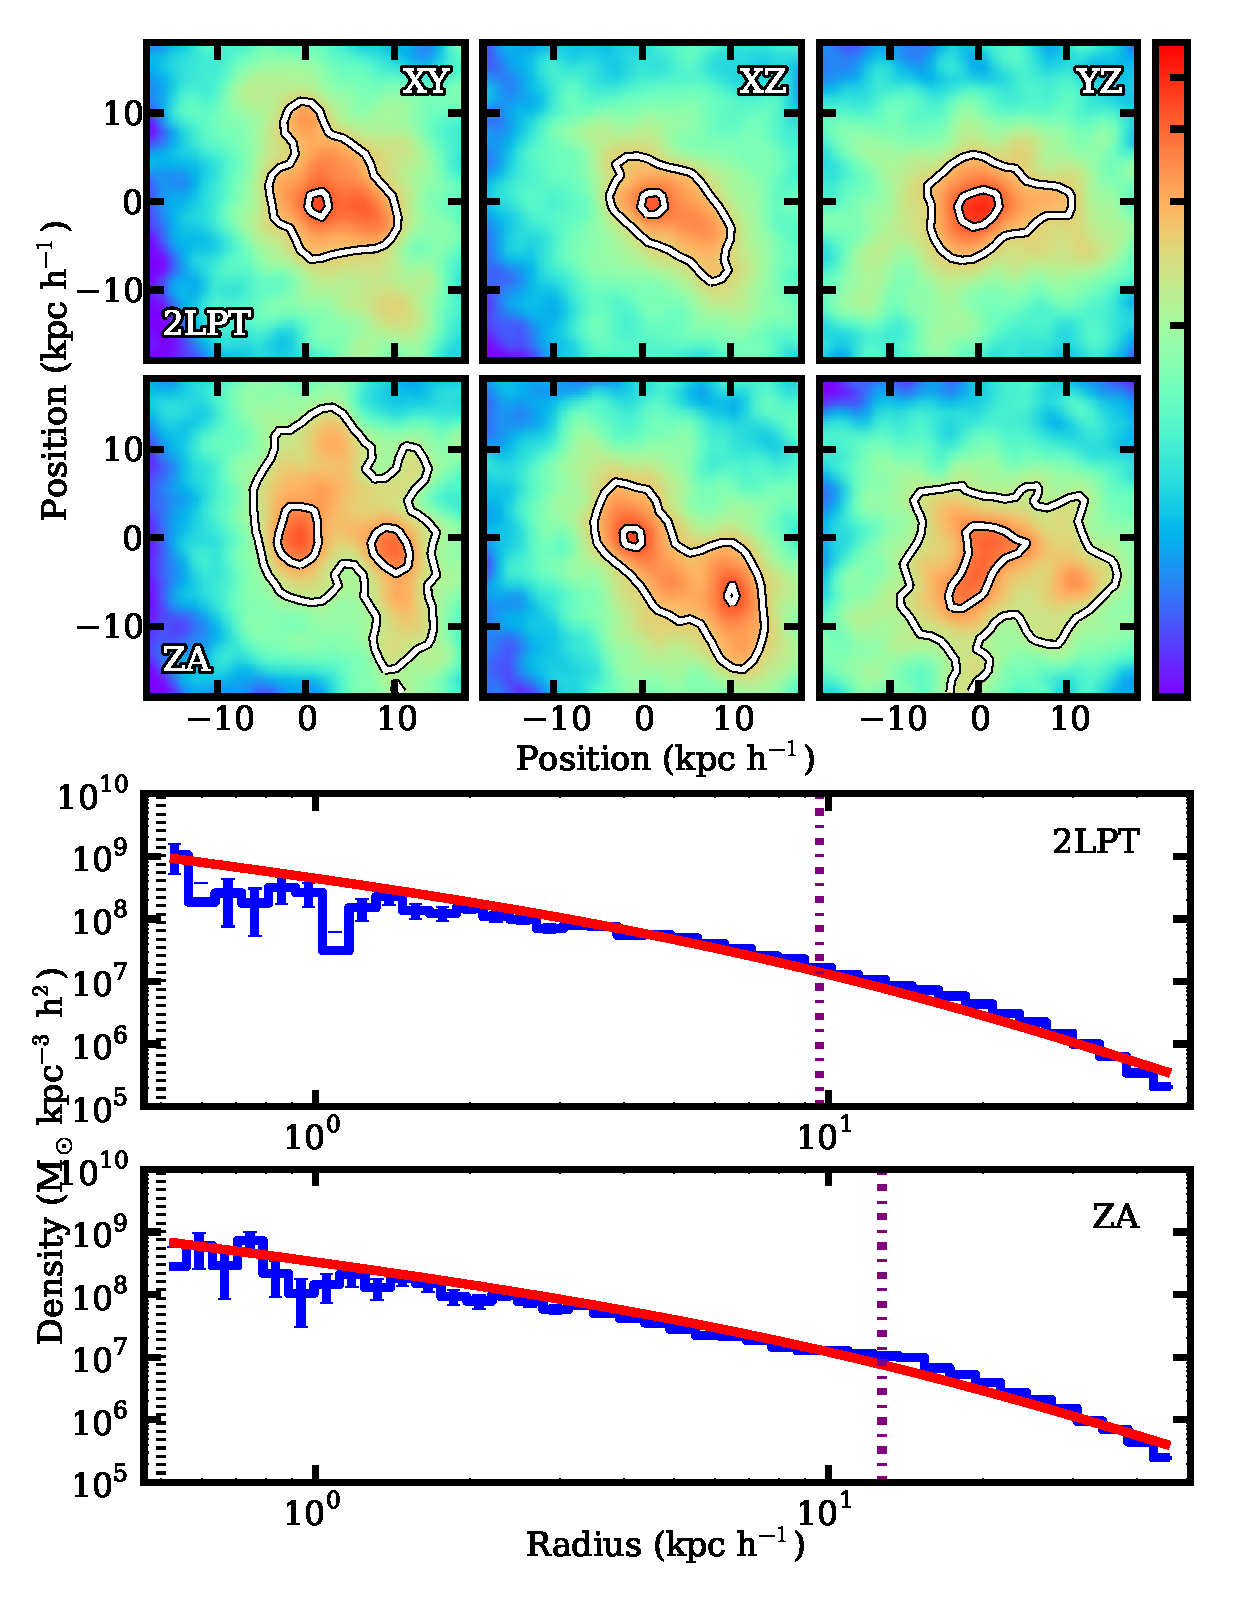
\includegraphics[width=\linewidth]{halo-pair_070_snap061.eps}
    \caption[Comparison of matched \lpt\ and \za\ halos]{\footnotesize \textit{Top two rows:}  Density projections for two matching halos at $z = 6$.  The first and second row are \lpt\ and \za, respectively.  The halos appear to be either undergoing or have recently undergone a major merger.  The \lpt\ halo appears to be more relaxed and further along in the merger process, while the \za\ halo lags behind, still displaying two distinct cores.  \textit{Bottom two rows:}  Density profiles for the same two halos as above.  NFW profiles are fit to logarithmic radial bins of particle position and are overplotted as red curves.  The purple dot--dash lines mark the scale radii.  The black dotted lines mark the resolution limit of the simulations.}
    \label{fig:halo-pair}
\end{figure}

Halo concentration $c=R_{vir}/R_{s}$ is derived from \rockstar's output for $R_{s}$ and $R_{vir}$, where $R_{s}$ is the scale radius defined by the NFW \citep{1996ApJ...462..563N} profile
\begin{equation} \label{eq:nfw_profile}
	\rho(r) = \frac{ \rho_{0} }{ \frac{ r }{ R_{s}} \left( 1 + \frac{r}{R_{s}} \right)^{2} }
\end{equation}
and $R_{vir}$ is the virial radius as defined by \citet{1998ApJ...495...80B}.  To verify the accuracy of the \rockstar\ fit, we independently find density profiles for several halos and compare the fit parameters such as $R_{s}$.  For each halo, we fit an NFW density profile to logarithmic radial bins of particle position with a non-linear least squares fitting routine from the SciPy library.  From this, we measure the scale radius and, along with virial radii from \rockstar, the concentration.  The bottom two rows of Figure~\ref{fig:halo-pair}, for example, show the fitting results for a particle matched halo pair.  For halos fit by our method, our results are in relatively good agreement with \rockstar.  However, as we do not find an acceptable fit for every halo, we use the more complete \rockstar\ data for the final concentration measurements.  However, we do note that \rockstar\ does not provide goodness-of-fit parameters for it's internal density profile measurements used to derive concentration, so error estimates for concentration values of individual halos are unknown.  Additionally, proper density profile fitting is non-trivial, as the non-linear interactions of numerical simulations rarely result in simple spherical halos that can be well described using spherical bins.

Figure~\ref{fig:halo-pair} also makes evident the difficulty in fitting density profiles and obtaining concentration measurements for typical realistic halos.  Large substructure, as displayed by the \za\ halo, can defeat the radial symmetry of the halo and cause significant deviations in the density profile.  Centering can also be an issue in these cases.  Due to these complications, there are a number of approaches for finding halo concentrations \citep{2012MNRAS.423.3018P}, but for consistency, we use the values derived from \rockstar's fitting for our concentration measurements.
